\documentclass[aspectratio=169]{beamer}


\usepackage{fontspec}
\usepackage{polyglossia}
\usepackage{color}
\setdefaultlanguage{russian}

\usetheme{metropolis}

\metroset{background=light}
\metroset{sectionpage=none}
\metroset{numbering=fraction}

\definecolor{ssaublue}{RGB}{77,144,205}
\setbeamercolor{frametitle}{fg=white, bg=ssaublue}
\setbeamercolor{title separator}{fg=ssaublue}
\setmainfont[
    Path = fonts/elektratextpro/,
    Extension = .otf,
    UprightFont = elektratextpro,
    BoldFont = elektratextpro_bold,
    ItalicFont = elektratextpro_italic
]{elektratextpro}

\setsansfont[
    Path = fonts/elektratextpro/,
    Extension = .otf,
    UprightFont = elektratextpro,
    BoldFont = elektratextpro_bold,
    ItalicFont = elektratextpro_italic
]{elektratextpro}

\setmonofont[
    Path = fonts/elektratextpro/,
    Extension = .otf,
    UprightFont = elektratextpro,
    BoldFont = elektratextpro_bold,
    ItalicFont = elektratextpro_italic
]{elektratextpro}

\newfontfamily\cyrillicfont[
    Path = fonts/elektratextpro/,
    Extension = .otf,
    UprightFont = elektratextpro,
    BoldFont = elektratextpro_bold,
    ItalicFont = elektratextpro_italic
]{elektratextpro}

\newfontfamily\cyrillicfontsf[
    Path = fonts/elektratextpro/,
    Extension = .otf,
    UprightFont = elektratextpro,
    BoldFont = elektratextpro_bold,
    ItalicFont = elektratextpro_italic
]{elektratextpro}

\newfontfamily\cyrillicfonttt[
    Path = fonts/elektratextpro/,
    Extension = .otf,
    UprightFont = elektratextpro,
    BoldFont = elektratextpro_bold,
    ItalicFont = elektratextpro_italic
]{elektratextpro}

\title{Пример презентации}
\author{Иван Иванов}
\date{\today}



\begin{document}

    \maketitle

    \begin{frame}{Заголовок}
        Это пример слайда на русском языке.
        Hello, world!
    \end{frame}

    \begin{frame}[fragile]{Пример}
        \metroset{block=fill}

        \begin{block}{Default}
            \begin{verbatim}
Block content.
Block content.
Block content.
Block content.
Block content.
            \end{verbatim}
        \end{block}
    \end{frame}

    {
        \setbeamertemplate{frame footer}{
            \scriptsize\href{https://example.com}{\textcolor{lightgray}{Тут ссылочка}}
        }
        \begin{frame}{А тут кастомный футер}
            Смотри ниже
        \end{frame}
    }

    \begin{frame}{Маркерованный список}
        \begin{itemize}
            \item Первый пункт
            \item Второй пункт
            \item Третий пункт
        \end{itemize}
    \end{frame}

    \begin{frame}{Нумерованный список}
        \begin{enumerate}
            \item Первый пункт
            \item Второй пункт
            \item Третий пункт
        \end{enumerate}
    \end{frame}

    \begin{frame}{Пример только с картинкой}
        \begin{figure}
            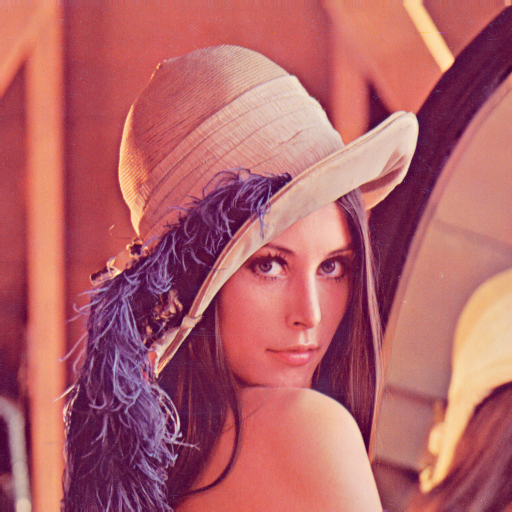
\includegraphics[width=0.4\textwidth]{images/Lenna}
            \caption{Lenna}
        \end{figure}

%        \begin{center}
%        \end{center}
    \end{frame}

    \begin{frame}{Пример с картинкой и текстом}
        \begin{columns}
            \column{0.4\textwidth}
            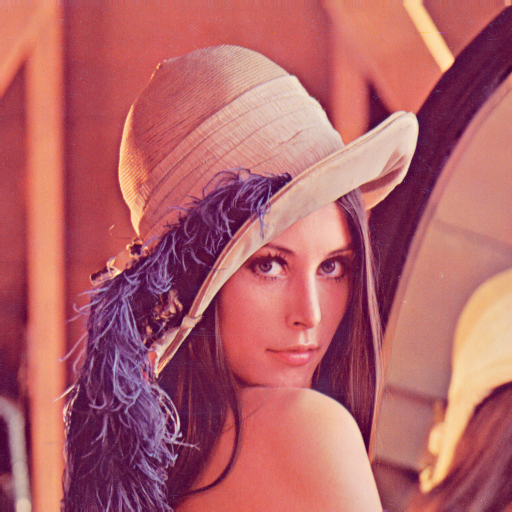
\includegraphics[width=\textwidth]{images/Lenna}
            \column{0.5\textwidth}
            Здесь ваш **текст**. Вы можете вставить списки, формулы, цитаты и т.д.
        \end{columns}
    \end{frame}

\end{document}
